
\columnratio{0.55}
\begin{paracol}{2}  
\switchcolumn[0]*%%%%%%%
\section{Using Vue with TypeScript}
\switchcolumn
\section{搭配 TypeScript 使用 Vue}
\switchcolumn[0]*%%%%%%%
A type system like TypeScript can detect many common errors via static
analysis at build time. This reduces the chance of runtime errors in
production, and also allows us to more confidently refactor code in
large-scale applications. TypeScript also improves developer ergonomics
via type-based auto-completion in IDEs.
\switchcolumn
像 TypeScript
这样的类型系统可以在编译时通过静态分析检测出很多常见错误。这减少了生产环境中的运行时错误,也让我们在重构大型项目的时候更有信心。通过
IDE 中基于类型的自动补全,TypeScript 还改善了开发体验和效率。
\switchcolumn[0]*%%%%%%%
Vue is written in TypeScript itself and provides first-class TypeScript
support. All official Vue packages come with bundled type declarations
that should work out-of-the-box.
\switchcolumn
Vue 本身就是用 TypeScript 编写的,并对 TypeScript
提供了一等公民的支持。所有的 Vue 官方库都自带了类型声明文件,开箱即用。
\switchcolumn[0]*%%%%%%%
\subsection{Project Setup}
\switchcolumn
\subsection{项目配置}
\switchcolumn[0]*%%%%%%%
\href{https://github.com/vuejs/create-vue}{\texttt{create-vue}}, the
official project scaffolding tool, offers the options to scaffold a
\href{https://vitejs.dev/}{Vite}-powered, TypeScript-ready Vue project.
\switchcolumn
\href{https://github.com/vuejs/create-vue}{\texttt{create-vue}},即官方的项目脚手架工具,提供了搭建基于
\href{https://cn.vitejs.dev/}{Vite} 且 TypeScript 就绪的 Vue
项目的选项。
\switchcolumn[0]*%%%%%%%
\subsubsection{Overview}
\switchcolumn
\subsubsection{总览}
\switchcolumn[0]*%%%%%%%
With a Vite-based setup, the dev server and the bundler are
transpilation-only and do not perform any type-checking. This ensures
the Vite dev server stays blazing fast even when using TypeScript.
\switchcolumn
在基于 Vite 的配置中,开发服务器和打包器将只会对 TypeScript
文件执行语法转译,而不会执行任何类型检查,这保证了 Vite 开发服务器在使用
TypeScript 时也能始终保持飞快的速度。
\switchcolumn[0]*%%%%%%%
\begin{itemize}
\item
  During development, we recommend relying on a good
  \href{https://vuejs.org/guide/typescript/overview.html\#ide-support}{IDE
  setup} for instant feedback on type errors.
\item
  If using SFCs, use the
  \href{https://github.com/vuejs/language-tools/tree/master/packages/tsc}{\texttt{vue-tsc}}
  utility for command line type checking and type declaration
  generation. \texttt{vue-tsc} is a wrapper around \texttt{tsc},
  TypeScript's own command line interface. It works largely the same as
  \texttt{tsc} except that it supports Vue SFCs in addition to
  TypeScript files. You can run \texttt{vue-tsc} in watch mode in
  parallel to the Vite dev server, or use a Vite plugin like
  \href{https://vite-plugin-checker.netlify.app/}{vite-plugin-checker}
  which runs the checks in a separate worker thread.
\item
  Vue CLI also provides TypeScript support, but is no longer
  recommended. See
  \href{https://vuejs.org/guide/typescript/overview.html\#note-on-vue-cli-and-ts-loader}{notes
  below}.
\end{itemize}
\switchcolumn
\begin{itemize}
\item
  在开发阶段,我们推荐你依赖一个好的
  \href{https://cn.vuejs.org/guide/typescript/overview.html\#ide-support}{IDE
  配置}来获取即时的类型错误反馈。
\item
  对于单文件组件,你可以使用工具
  \href{https://github.com/vuejs/language-tools/tree/master/packages/tsc}{\texttt{vue-tsc}}
  在命令行检查类型和生成类型声明文件。\texttt{vue-tsc} 是对 TypeScript
  自身命令行界面 \texttt{tsc} 的一个封装。它的工作方式基本和
  \texttt{tsc} 一致。除了 TypeScript 文件,它还支持 Vue
  的单文件组件。你可以在开启 Vite 开发服务器的同时以侦听模式运行
  \texttt{vue-tsc},或是使用
  \href{https://vite-plugin-checker.netlify.app/}{vite-plugin-checker}
  这样在另一个 worker 线程里做静态检查的插件。
\item
  Vue CLI 也提供了对 TypeScript
  的支持,但是已经不推荐了。详见\href{https://cn.vuejs.org/guide/typescript/overview.html\#note-on-vue-cli-and-ts-loader}{下方的说明}。
\end{itemize}
\end{paracol}



\columnratio{0.55}
\begin{paracol}{2} 
 
\switchcolumn[0]*%%%%%%%
\subsubsection{IDE Support}
\switchcolumn
\subsubsection{IDE 支持}
\switchcolumn[0]*%%%%%%%
\begin{itemize}
\item
  \href{https://code.visualstudio.com/}{Visual Studio Code} (VSCode) is
  strongly recommended for its great out-of-the-box support for
  TypeScript.
  \begin{itemize}
  \item
    \href{https://marketplace.visualstudio.com/items?itemName=Vue.volar}{Volar}
    is the official VSCode extension that provides TypeScript support
    inside Vue SFCs, along with many other great features.
\begin{vueQuote}{TIP}
    Volar replaces
    \href{https://marketplace.visualstudio.com/items?itemName=octref.vetur}{Vetur},
    our previous official VSCode extension for Vue 2. If you have Vetur
    currently installed, make sure to disable it in Vue 3 projects.
\end{vueQuote} 
  \item
    \href{https://marketplace.visualstudio.com/items?itemName=Vue.vscode-typescript-vue-plugin}{TypeScript
    Vue Plugin} is also needed to get type support for \texttt{*.vue}
    imports in TS files.
  \end{itemize}
\item
  \href{https://www.jetbrains.com/webstorm/}{WebStorm} also provides
  out-of-the-box support for both TypeScript and Vue. Other JetBrains
  IDEs support them too, either out of the box or via
  \href{https://plugins.jetbrains.com/plugin/9442-vue-js}{a free
  plugin}. As of version 2023.2, WebStorm and the Vue Plugin come with
  built-in support for the Vue Language Server. You can set the Vue
  service to use Volar integration on all TypeScript versions, under
  Settings \textgreater{} Languages \& Frameworks \textgreater{}
  TypeScript \textgreater{} Vue. By default, Volar will be used for
  TypeScript versions 5.0 and higher.
\end{itemize}
\switchcolumn
\begin{itemize}
\item
  强烈推荐 \href{https://code.visualstudio.com/}{Visual Studio Code}
  (VSCode),因为它对 TypeScript 有着很好的内置支持。
  \begin{itemize}
  \item
    \href{https://marketplace.visualstudio.com/items?itemName=Vue.volar}{Volar}
    是官方的 VSCode 扩展,提供了 Vue 单文件组件中的 TypeScript
    支持,还伴随着一些其他非常棒的特性。
\begin{vueQuote}{TIP}
    Volar 取代了我们之前为 Vue 2 提供的官方 VSCode 扩展
    \href{https://marketplace.visualstudio.com/items?itemName=octref.vetur}{Vetur}。如果你之前已经安装了
    Vetur,请确保在 Vue 3 的项目中禁用它。
\end{vueQuote} 
  \item
    \href{https://marketplace.visualstudio.com/items?itemName=Vue.vscode-typescript-vue-plugin}{TypeScript
    Vue Plugin} 用于支持在 TS 中 import \texttt{*.vue} 文件。
  \end{itemize}
\item
  \href{https://www.jetbrains.com/webstorm/}{WebStorm} 对 TypeScript 和
  Vue 也都提供了开箱即用的支持。其他的 JetBrains IDE
  也同样可以通过一个\href{https://plugins.jetbrains.com/plugin/9442-vue-js}{免费插件}支持。从
  2023.2 版开始,WebStorm 和 Vue 插件内置了对 Vue
  语言服务器的支持。你可以在设置 \textgreater{} 语言和框架
  \textgreater{} TypeScript \textgreater{} Vue 下将 Vue 服务设置为在所有
  TypeScript 版本上使用 Volar 集成。默认情况下,Volar 将用于 TypeScript
  5.0 及更高版本。
\end{itemize}
\end{paracol}


\columnratio{0.55}
\begin{paracol}{2} 
 
\switchcolumn[0]*%%%%%%%
\subsubsection{Configuring tsconfig.json}
\switchcolumn
\subsubsection{配置 tsconfig.json}
\switchcolumn[0]*%%%%%%%
Projects scaffolded via \texttt{create-vue} include pre-configured
\texttt{tsconfig.json}. The base config is abstracted in the
\href{https://github.com/vuejs/tsconfig}{\texttt{@vue/tsconfig}}
package. Inside the project, we use
\href{https://www.typescriptlang.org/docs/handbook/project-references.html}{Project
References} to ensure correct types for code running in different
environments (e.g. app code and test code should have different global
variables).
\switchcolumn
通过 \texttt{create-vue} 搭建的项目包含了预先配置好的
\texttt{tsconfig.json}。其底层配置抽象于
\href{https://github.com/vuejs/tsconfig}{\texttt{@vue/tsconfig}}
包中。在项目内我们使用
\href{https://www.typescriptlang.org/docs/handbook/project-references.html}{Project
References} 来确保运行在不同环境下的代码的类型正确
(比如应用代码和测试代码应该有不同的全局变量)。
\switchcolumn[0]*%%%%%%%
When configuring \texttt{tsconfig.json} manually, some notable options
include:
\switchcolumn
手动配置 \texttt{tsconfig.json} 时,请留意以下选项:
\switchcolumn[0]*%%%%%%%
\begin{itemize}
\item
  \href{https://www.typescriptlang.org/tsconfig\#isolatedModules}{\texttt{compilerOptions.isolatedModules}}
  is set to \texttt{true} because Vite uses
  \href{https://esbuild.github.io/}{esbuild} for transpiling TypeScript
  and is subject to single-file transpile limitations.
\item
  If you're using Options API, you need to set
  \href{https://www.typescriptlang.org/tsconfig\#strict}{\texttt{compilerOptions.strict}}
  to \texttt{true} (or at least enable
  \href{https://www.typescriptlang.org/tsconfig\#noImplicitThis}{\texttt{compilerOptions.noImplicitThis}},
  which is a part of the \texttt{strict} flag) to leverage type checking
  of \texttt{this} in component options. Otherwise \texttt{this} will be
  treated as \texttt{any}.
\item
  If you have configured resolver aliases in your build tool, for
  example the \texttt{@/*} alias configured by default in a
  \texttt{create-vue} project, you need to also configure it for
  TypeScript via
  \href{https://www.typescriptlang.org/tsconfig\#paths}{\texttt{compilerOptions.paths}}.
\end{itemize}
\switchcolumn
\begin{itemize}
\item
  \href{https://www.typescriptlang.org/tsconfig\#isolatedModules}{\texttt{compilerOptions.isolatedModules}}
  应当设置为 \texttt{true},因为 Vite 使用
  \href{https://esbuild.github.io/}{esbuild} 来转译
  TypeScript,并受限于单文件转译的限制。
\item
  如果你正在使用选项式 API,需要将
  \href{https://www.typescriptlang.org/tsconfig\#strict}{\texttt{compilerOptions.strict}}
  设置为 \texttt{true} (或者至少开启
  \href{https://www.typescriptlang.org/tsconfig\#noImplicitThis}{\texttt{compilerOptions.noImplicitThis}},它是
  \texttt{strict} 模式的一部分),才可以获得对组件选项中 \texttt{this}
  的类型检查。否则 \texttt{this} 会被认为是 \texttt{any}。
\item
  如果你在构建工具中配置了路径解析别名,例如 \texttt{@/*}
  这个别名被默认配置在了 \texttt{create-vue} 项目中,你需要通过
  \href{https://www.typescriptlang.org/tsconfig\#paths}{\texttt{compilerOptions.paths}}
  选项为 TypeScript 再配置一遍。
\end{itemize}
\switchcolumn[0]*%%%%%%%
See also:
\switchcolumn
参考:
\switchcolumn[0]*%%%%%%%
\begin{itemize}
\item
  \href{https://www.typescriptlang.org/docs/handbook/compiler-options.html}{Official
  TypeScript compiler options docs}
\item
  \href{https://esbuild.github.io/content-types/\#typescript-caveats}{esbuild
  TypeScript compilation caveats}
\end{itemize}
\switchcolumn
\begin{itemize}
\item
  \href{https://www.typescriptlang.org/docs/handbook/compiler-options.html}{官方
  TypeScript 编译选项文档}
\item
  \href{https://esbuild.github.io/content-types/\#typescript-caveats}{esbuild
  TypeScript 编译注意事项}
\end{itemize}
\end{paracol}



\columnratio{0.55}
\begin{paracol}{2} 
 
\switchcolumn[0]*%%%%%%%
\subsubsection{Volar Takeover Mode}
\switchcolumn
\subsubsection{Volar Takeover 模式}
\switchcolumn[0]*%%%%%%%
\begin{quote}
This section only applies for VSCode + Volar.
\end{quote}
\switchcolumn
\begin{quote}
这一章节仅针对 VSCode + Volar。
\end{quote}
\switchcolumn[0]*%%%%%%%
To get Vue SFCs and TypeScript working together, Volar creates a
separate TS language service instance patched with Vue-specific support,
and uses it in Vue SFCs. At the same time, plain TS files are still
handled by VSCode's built-in TS language service, which is why we need
\href{https://marketplace.visualstudio.com/items?itemName=Vue.vscode-typescript-vue-plugin}{TypeScript
Vue Plugin} to support Vue SFC imports in TS files. This default setup
works, but for each project we are running two TS language service
instances: one from Volar, one from VSCode's built-in service. This is a
bit inefficient and can lead to performance issues in large projects.
\switchcolumn
为了让 Vue 单文件组件和 TypeScript 一起工作,Volar 创建了一个针对 Vue 的
TS 语言服务实例,将其用于 Vue 单文件组件。同时,普通的 TS 文件依然由
VSCode 内置的 TS 语言服务来处理。这也是为什么我们需要安装
\href{https://marketplace.visualstudio.com/items?itemName=Vue.vscode-typescript-vue-plugin}{TypeScript
Vue Plugin} 来支持在 TS 文件中引入 Vue
单文件组件。这套默认设置能够工作,但在每个项目里我们都运行了两个语言服务实例:一个来自
Volar,一个来自 VSCode
的内置服务。这在大型项目里可能会带来一些性能问题。
\switchcolumn[0]*%%%%%%%
Volar provides a feature called "Takeover Mode" to improve performance.
In takeover mode, Volar provides support for both Vue and TS files using
a single TS language service instance.
\switchcolumn
为了优化性能,Volar 提供了一个叫做``Takeover
模式''的功能。在这个模式下,Volar 能够使用一个 TS 语言服务实例同时为 Vue
和 TS 文件提供支持。
\switchcolumn[0]*%%%%%%%
To enable Takeover Mode, you need to disable VSCode's built-in TS
language service in \textbf{your project's workspace only} by following
these steps:
\switchcolumn
要开启 Takeover
模式,你需要执行以下步骤来\textbf{在你的项目的工作空间中}禁用 VSCode
的内置 TS 语言服务:
\switchcolumn[0]*%%%%%%%
\begin{enumerate}
\item
  In your project workspace, bring up the command palette with
  \texttt{Ctrl\ +\ Shift\ +\ P} (macOS: \texttt{Cmd\ +\ Shift\ +\ P}).
\item
  Type \texttt{built} and select "Extensions: Show Built-in Extensions".
\item
  Type \texttt{typescript} in the extension search box (do not remove
  \texttt{@builtin} prefix).
\item
  Click the little gear icon of "TypeScript and JavaScript Language
  Features", and select "Disable (Workspace)".
\item
  Reload the workspace. Takeover mode will be enabled when you open a
  Vue or TS file.
\end{enumerate}
\switchcolumn
\begin{enumerate}
\item
  在当前项目的工作空间下,用 \texttt{Ctrl\ +\ Shift\ +\ P}
  (macOS:\texttt{Cmd\ +\ Shift\ +\ P}) 唤起命令面板。
\item
  输入 \texttt{built},然后选择``Extensions:Show Built-in
  Extensions''。
\item
  在插件搜索框内输入 \texttt{typescript} (不要删除 \texttt{@builtin}
  前缀)。
\item
  点击``TypeScript and JavaScript Language
  Features''右下角的小齿轮,然后选择``Disable (Workspace)''。
\item
  重新加载工作空间。Takeover 模式将会在你打开一个 Vue 或者 TS
  文件时自动启用。
\end{enumerate}
\end{paracol}

\begin{center} 
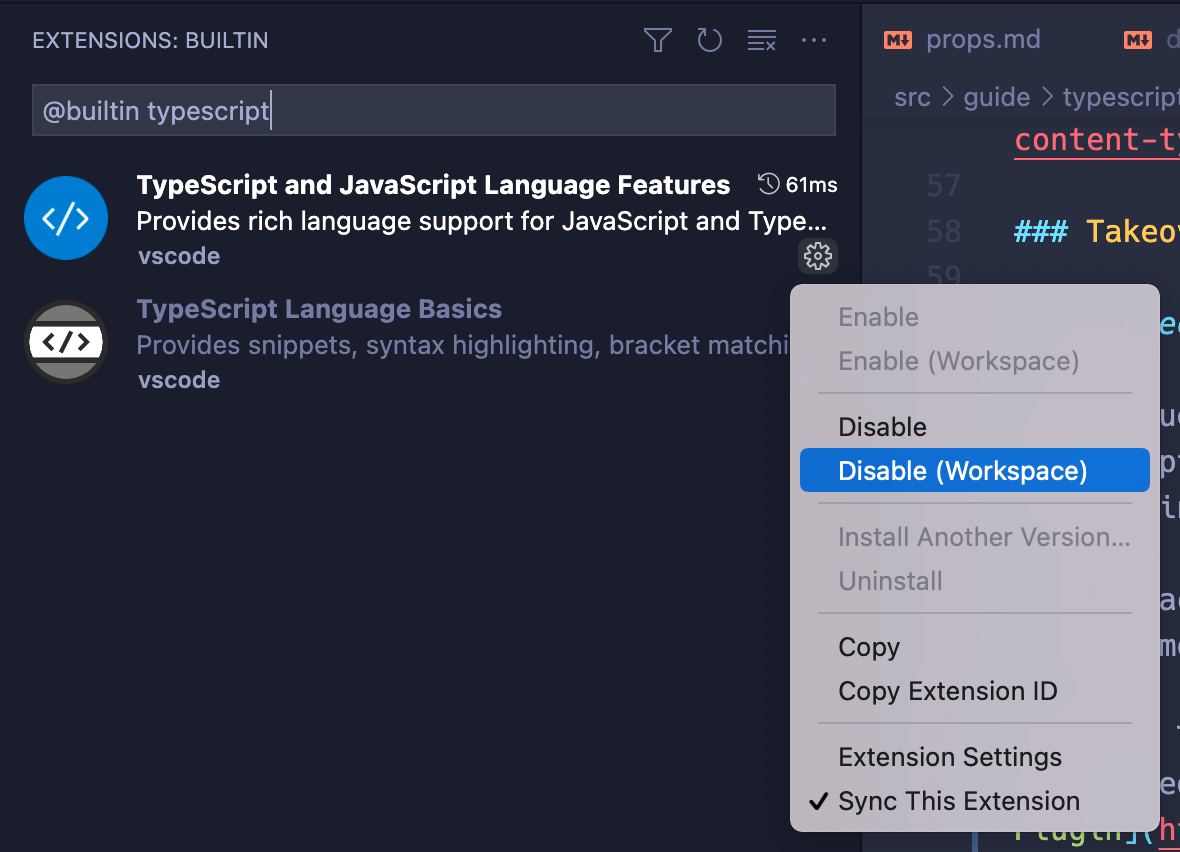
\includegraphics{./img/takeover-mode.54f7bbf6.png} 
\end{center}


\columnratio{0.55}
\begin{paracol}{2} 
 
\switchcolumn[0]*%%%%%%%
\subsubsection{Note on Vue CLI and ts-loader}
\switchcolumn
\subsubsection{关于 Vue CLI 和 ts-loader}
\switchcolumn[0]*%%%%%%%
In webpack-based setups such as Vue CLI, it is common to perform type
checking as part of the module transform pipeline, for example with
\texttt{ts-loader}. This, however, isn't a clean solution because the
type system needs knowledge of the entire module graph to perform type
checks. Individual module's transform step simply is not the right place
for the task. It leads to the following problems:
\switchcolumn
像 Vue CLI 这样的基于 webpack
搭建的项目,通常是在模块编译的过程中顺道执行类型检查,例如使用
\texttt{ts-loader}。然而这并不是一个理想的解决方案,因为类型系统需要了解整个模块关系才能执行类型检查。loader
中只适合单个模块的编译,并不适合做需要全局信息的工作。这导致了下面的问题:
\switchcolumn[0]*%%%%%%%
\begin{itemize}
\item
  \texttt{ts-loader} can only type check post-transform code. This
  doesn't align with the errors we see in IDEs or from \texttt{vue-tsc},
  which map directly back to the source code.
\item
  Type checking can be slow. When it is performed in the same thread /
  process with code transformations, it significantly affects the build
  speed of the entire application.
\item
  We already have type checking running right in our IDE in a separate
  process, so the cost of dev experience slow down simply isn't a good
  trade-off.
\end{itemize}
\switchcolumn
\begin{itemize}
\item
  \texttt{ts-loader} 只能对在它之前的 loader
  编译转换后的代码执行类型检查,这和我们在 IDE 或 \texttt{vue-tsc}
  中看到的基于源代码的错误提示并不一致。
\item
  类型检查可能会很慢。当它和代码转换在相同的线程/进程中执行时,它会显著影响整个应用的构建速度。
\item
  我们已经在 IDE
  中通过单独的进程运行着类型检查了,却还要在构建流程中执行类型检查导致降低开发体验,这似乎不太划算。
\end{itemize}
\switchcolumn[0]*%%%%%%%
If you are currently using Vue 3 + TypeScript via Vue CLI, we strongly
recommend migrating over to Vite. We are also working on CLI options to
enable transpile-only TS support, so that you can switch to
\texttt{vue-tsc} for type checking.
\switchcolumn
如果你正通过 Vue CLI 使用 Vue 3 和 TypeScript,我们强烈建议你迁移到
Vite。我们也在为 CLI 开发仅执行 TS 语法转译的选项,以允许你切换至
\texttt{vue-tsc} 来执行类型检查。
\end{paracol}



\columnratio{0.55}
\begin{paracol}{2} 
 
\switchcolumn[0]*%%%%%%%
\subsection{General Usage Notes}
\switchcolumn
\subsection{常见使用说明}
\switchcolumn[0]*%%%%%%%
\subsubsection{defineComponent()}
\switchcolumn
\subsubsection{defineComponent()}
\switchcolumn[0]*%%%%%%%
To let TypeScript properly infer types inside component options, we need
to define components with
\href{https://vuejs.org/api/general.html\#definecomponent}{\texttt{defineComponent()}}:
\switchcolumn
为了让 TypeScript 正确地推导出组件选项内的类型,我们需要通过
\href{https://cn.vuejs.org/api/general.html\#definecomponent}{\texttt{defineComponent()}}
这个全局 API 来定义组件:
\switchcolumn[0]*%%%%%%%
\begin{codeJs}
import { defineComponent } from 'vue'
export default defineComponent({
  // 启用了类型推导
  props: {
    name: String,
    msg: { type: String, required: true }
  },
  data() {
    return {
      count: 1
    }
  },
  mounted() {
    this.name // 类型:string | undefined
    this.msg // 类型:string
    this.count // 类型:number
  }
})
\end{codeJs}
\switchcolumn
\begin{codeJs}
import { defineComponent } from 'vue'
export default defineComponent({
  // 启用了类型推导
  props: {
    name: String,
    msg: { type: String, required: true }
  },
  data() {
    return {
      count: 1
    }
  },
  mounted() {
    this.name // 类型:string | undefined
    this.msg // 类型:string
    this.count // 类型:number
  }
})
\end{codeJs}
\switchcolumn[0]*%%%%%%%
\texttt{defineComponent()} also supports inferring the props passed to
\texttt{setup()} when using Composition API without
\texttt{\textless{}script\ setup\textgreater{}}:
\switchcolumn
当没有结合 \texttt{\textless{}script\ setup\textgreater{}} 使用组合式
API 时,\texttt{defineComponent()} 也支持对传递给 \texttt{setup()} 的
prop 的推导:
\switchcolumn[0]*%%%%%%%
\begin{codeJs}
import { defineComponent } from 'vue'
export default defineComponent({
  // 启用了类型推导
  props: {
    message: String
  },
  setup(props) {
    props.message // 类型:string | undefined
  }
})
\end{codeJs}
\switchcolumn
\begin{codeJs}
import { defineComponent } from 'vue'
export default defineComponent({
  // 启用了类型推导
  props: {
    message: String
  },
  setup(props) {
    props.message // 类型:string | undefined
  }
})
\end{codeJs}
\switchcolumn[0]*%%%%%%%
See also:
\switchcolumn
参考:
\switchcolumn[0]*%%%%%%%
\begin{itemize}
\item
  \href{https://vuejs.org/api/general.html\#note-on-webpack-treeshaking}{Note
  on webpack Treeshaking}
\item
  \href{https://github.com/vuejs/core/blob/main/packages/dts-test/defineComponent.test-d.tsx}{type
  tests for \texttt{defineComponent}}
\end{itemize}
\switchcolumn
\begin{itemize}
\item
  \href{https://cn.vuejs.org/api/general.html\#note-on-webpack-treeshaking}{webpack
  Treeshaking 的注意事项}
\item
  \href{https://github.com/vuejs/core/blob/main/packages/dts-test/defineComponent.test-d.tsx}{对
  \texttt{defineComponent} 的类型测试}
\end{itemize}
\switchcolumn[0]*%%%%%%%
\begin{vueQuote}{TIP}
\texttt{defineComponent()} also enables type inference for components
defined in plain JavaScript.
\end{vueQuote} 
\switchcolumn
\begin{vueQuote}{TIP}
\texttt{defineComponent()} 也支持对纯 JavaScript
编写的组件进行类型推导。
\end{vueQuote} 
\switchcolumn[0]*%%%%%%%
\subsubsection{Usage in Single-File Components}
\switchcolumn
\subsubsection{在单文件组件中的用法}
\switchcolumn[0]*%%%%%%%
To use TypeScript in SFCs, add the \texttt{lang="ts"} attribute to
\texttt{\textless{}script\textgreater{}} tags. When \texttt{lang="ts"}
is present, all template expressions also enjoy stricter type checking.
\switchcolumn
要在单文件组件中使用 TypeScript,需要在
\texttt{\textless{}script\textgreater{}} 标签上加上 \texttt{lang="ts"}
的 attribute。当 \texttt{lang="ts"}
存在时,所有的模板内表达式都将享受到更严格的类型检查。
\switchcolumn[0]*%%%%%%%
\begin{codeHtml}
<script lang="ts">
import { defineComponent } from 'vue'
export default defineComponent({
  data() {
    return {
      count: 1
    }
  }
})
</script>
<template>
  <!-- 启用了类型检查和自动补全 -->
  {{ count.toFixed(2) }}
</template>
\end{codeHtml}
\switchcolumn
\begin{codeHtml}
<script lang="ts">
import { defineComponent } from 'vue'
export default defineComponent({
  data() {
    return {
      count: 1
    }
  }
})
</script>
<template>
  <!-- 启用了类型检查和自动补全 -->
  {{ count.toFixed(2) }}
</template>
\end{codeHtml}
\switchcolumn[0]*%%%%%%%
\texttt{lang="ts"} can also be used with
\texttt{\textless{}script\ setup\textgreater{}}:
\switchcolumn
\texttt{lang="ts"} 也可以用于
\texttt{\textless{}script\ setup\textgreater{}}:
\switchcolumn[0]*%%%%%%%
\begin{codeHtml}
<script setup lang="ts">
// 启用了 TypeScript
import { ref } from 'vue'
const count = ref(1)
</script>
<template>
  <!-- 启用了类型检查和自动补全 -->
  {{ count.toFixed(2) }}
</template>
\end{codeHtml}
\switchcolumn
\begin{codeHtml}
<script setup lang="ts">
// 启用了 TypeScript
import { ref } from 'vue'
const count = ref(1)
</script>
<template>
  <!-- 启用了类型检查和自动补全 -->
  {{ count.toFixed(2) }}
</template>
\end{codeHtml}
\end{paracol}


\columnratio{0.55}
\begin{paracol}{2} 
 
\switchcolumn[0]*%%%%%%%
\subsubsection{TypeScript in Templates}
\switchcolumn
\subsubsection{模板中的 TypeScript}
\switchcolumn[0]*%%%%%%%
The \texttt{\textless{}template\textgreater{}} also supports TypeScript
in binding expressions when
\texttt{\textless{}script\ lang="ts"\textgreater{}} or
\texttt{\textless{}script\ setup\ lang="ts"\textgreater{}} is used. This
is useful in cases where you need to perform type casting in template
expressions.
\switchcolumn
在使用了 \texttt{\textless{}script\ lang="ts"\textgreater{}} 或
\texttt{\textless{}script\ setup\ lang="ts"\textgreater{}}
后,\texttt{\textless{}template\textgreater{}} 在绑定表达式中也支持
TypeScript。这对需要在模板表达式中执行类型转换的情况下非常有用。
\switchcolumn[0]*%%%%%%%
Here's a contrived example:
\switchcolumn
这里有一个假想的例子:
\switchcolumn[0]*%%%%%%%
\begin{codeHtml}
<script setup lang="ts">
let x: string | number = 1
</script>
<template>
  <!-- 出错,因为 x 可能是字符串 -->
  {{ x.toFixed(2) }}
</template>
\end{codeHtml}
\switchcolumn
\begin{codeHtml}
<script setup lang="ts">
let x: string | number = 1
</script>
<template>
  <!-- 出错,因为 x 可能是字符串 -->
  {{ x.toFixed(2) }}
</template>
\end{codeHtml}
\switchcolumn[0]*%%%%%%%
This can be worked around with an inline type cast:
\switchcolumn
可以使用内联类型强制转换解决此问题:
\switchcolumn[0]*%%%%%%%
\begin{codeHtml}
<script setup lang="ts">
let x: string | number = 1
</script>
<template>
  {{ (x as number).toFixed(2) }}
</template>
\end{codeHtml}
\switchcolumn
\begin{codeHtml}
<script setup lang="ts">
let x: string | number = 1
</script>
<template>
  {{ (x as number).toFixed(2) }}
</template>
\end{codeHtml}
\switchcolumn[0]*%%%%%%%
\begin{vueQuote}{TIP}
If using Vue CLI or a webpack-based setup, TypeScript in template
expressions requires \texttt{vue-loader@\^{}16.8.0}.
\end{vueQuote} 
\switchcolumn
\begin{vueQuote}{TIP}
如果正在使用 Vue CLI 或基于 webpack 的配置,支持模板内表达式的
TypeScript 需要 \texttt{vue-loader@\^{}16.8.0}。
\end{vueQuote} 
\end{paracol}



\columnratio{0.55}
\begin{paracol}{2} 
 
\switchcolumn[0]*%%%%%%%
\subsubsection{Usage with TSX}
\switchcolumn
\subsubsection{使用 TSX}
\switchcolumn[0]*%%%%%%%
Vue also supports authoring components with JSX / TSX. Details are
covered in the
\href{https://vuejs.org/guide/extras/render-function.html\#jsx-tsx}{Render
Function \& JSX} guide.
\switchcolumn
Vue 也支持使用 JSX / TSX
编写组件。详情请查阅\href{https://cn.vuejs.org/guide/extras/render-function.html\#jsx-tsx}{渲染函数
\& JSX}。
\switchcolumn[0]*%%%%%%%
\subsection{Generic Components}
\switchcolumn
\subsection{泛型组件}
\switchcolumn[0]*%%%%%%%
Generic components are supported in two cases:
\switchcolumn
泛型组件支持两种使用方式:
\switchcolumn[0]*%%%%%%%
\begin{itemize}
\item
  In SFCs:
  \href{https://vuejs.org/api/sfc-script-setup.html\#generics}{\texttt{\textasciigrave{}\ with\ the}generic`
  attribute}
\item
  Render function / JSX components:
  \href{https://vuejs.org/api/general.html\#function-signature}{\texttt{defineComponent()}'s
  function signature}
\end{itemize}
\switchcolumn
\begin{itemize}
\item
  在单文件组件中:\href{https://cn.vuejs.org/api/sfc-script-setup.html\#generics}{在
  \texttt{\textasciigrave{}\ 上使用}generic` 属性}
\item
  渲染函数 / JSX
  组件:\href{https://cn.vuejs.org/api/general.html\#function-signature}{\texttt{defineComponent()}
  的函数签名}
\end{itemize}
\switchcolumn[0]*%%%%%%%
\subsection{API-Specific Recipes}
\switchcolumn
\subsection{特定 API 的使用指南}
\switchcolumn[0]*%%%%%%%
\begin{itemize}
\item
  \href{https://vuejs.org/guide/typescript/composition-api.html}{TS with
  Composition API}
\item
  \href{https://vuejs.org/guide/typescript/options-api.html}{TS with
  Options API}
\end{itemize}
\switchcolumn
\begin{itemize}
\item
  \href{https://cn.vuejs.org/guide/typescript/composition-api.html}{TS
  与组合式 API}
\item
  \href{https://cn.vuejs.org/guide/typescript/options-api.html}{TS
  与选项式 API}
\end{itemize}
\end{paracol}

 